\chapter{Related Work}

In this section we present recent work related to convolutional RBMs which already have been proposed in discrete time.
We further show recent approaches for sampling and implementing Boltzmann machines in spiking neural networks.

\section{Convolutional RBM}

The convolutional RBM (cRBM) was invented more or less at the same time by Desjardins et al., Lee et al. and Norouzi et al. in 2008/2009 \cite{desjardins2008empirical}\cite{lee2009convolutional}\cite{norouzi2009stacks}. 
In similarity to CNNs it can be seen as the advancement of an energy based model adapting to compositional data.
Describing images in terms of spatially local features needs fewer parameters, generalizes better, and offers re-usability as identical local features can be extracted from different locations of an image.
Modelled after CNNs and unlike a normal RBM, the visible and hidden layer in the cRBM are connected in a convolutional manner (as described in section 2.x) instead of being fully connected.


Propagating information up can be seen as the convolution with a filter matrix $W$ (see Fig \ref{fig:convrbmsub1}): 
\[
P(\textbf{h} | \textbf{v}) = \sigma((W * \textbf{v}) + \textbf{b}_{h}).
\]
The down propagation utilizes the flipped kernel $\tilde{W}$  (see Fig \ref{fig:convrbmsub2} \& \ref{fig:convrbmsub3} ):
\[
P(\textbf{v}| \textbf{h}) = \sigma((\tilde{W} * \textbf{h}) + b_v).
\]
Using the convolution operation, the energy of the network can thus be rewritten as
\[
E(\textbf{h} , \textbf{v}) = \textbf{h}^\intercal(W * \textbf{v}) + \textbf{h}^\intercal \textbf{b}_{h} + \sum b v_i.
\]

%\begin{figure}
%	\centering
%	\begin{subfigure}[t]{.30\textwidth}
%  		\centering
%  		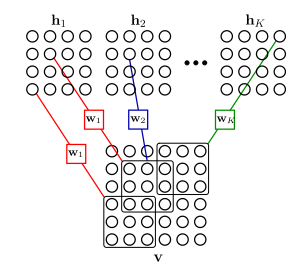
\includegraphics[width=.8\linewidth]{imgs/crbm1.png}
%  		\caption{A subfigure}
%  		\label{fig:sub1}
%	\end{subfigure}%
%	\begin{subfigure}[t]{.30\textwidth}
%  		\centering
%  		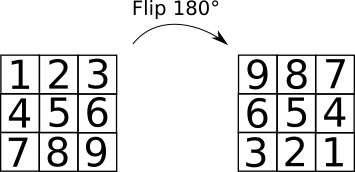
\includegraphics[width=.8\linewidth]{imgs/kernel_flip.png}
%  		\caption{A subfigure}
%  		\label{fig:sub2}
%	\end{subfigure}
%	\begin{subfigure}[t]{.30\textwidth}
%  		\centering
%  		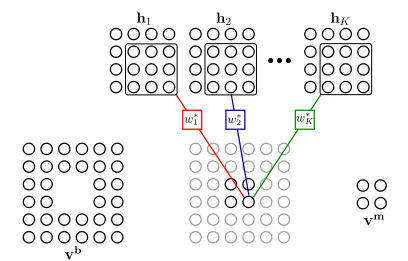
\includegraphics[width=.8\linewidth]{imgs/crbm2.png}
%  		\caption{A subfigure}
%  		\label{fig:sub3}
%	\end{subfigure}
%\end{figure}


\begin{figure}
	\centering
	\begin{subfigure}[t]{.30\textwidth}
  		\centering
  		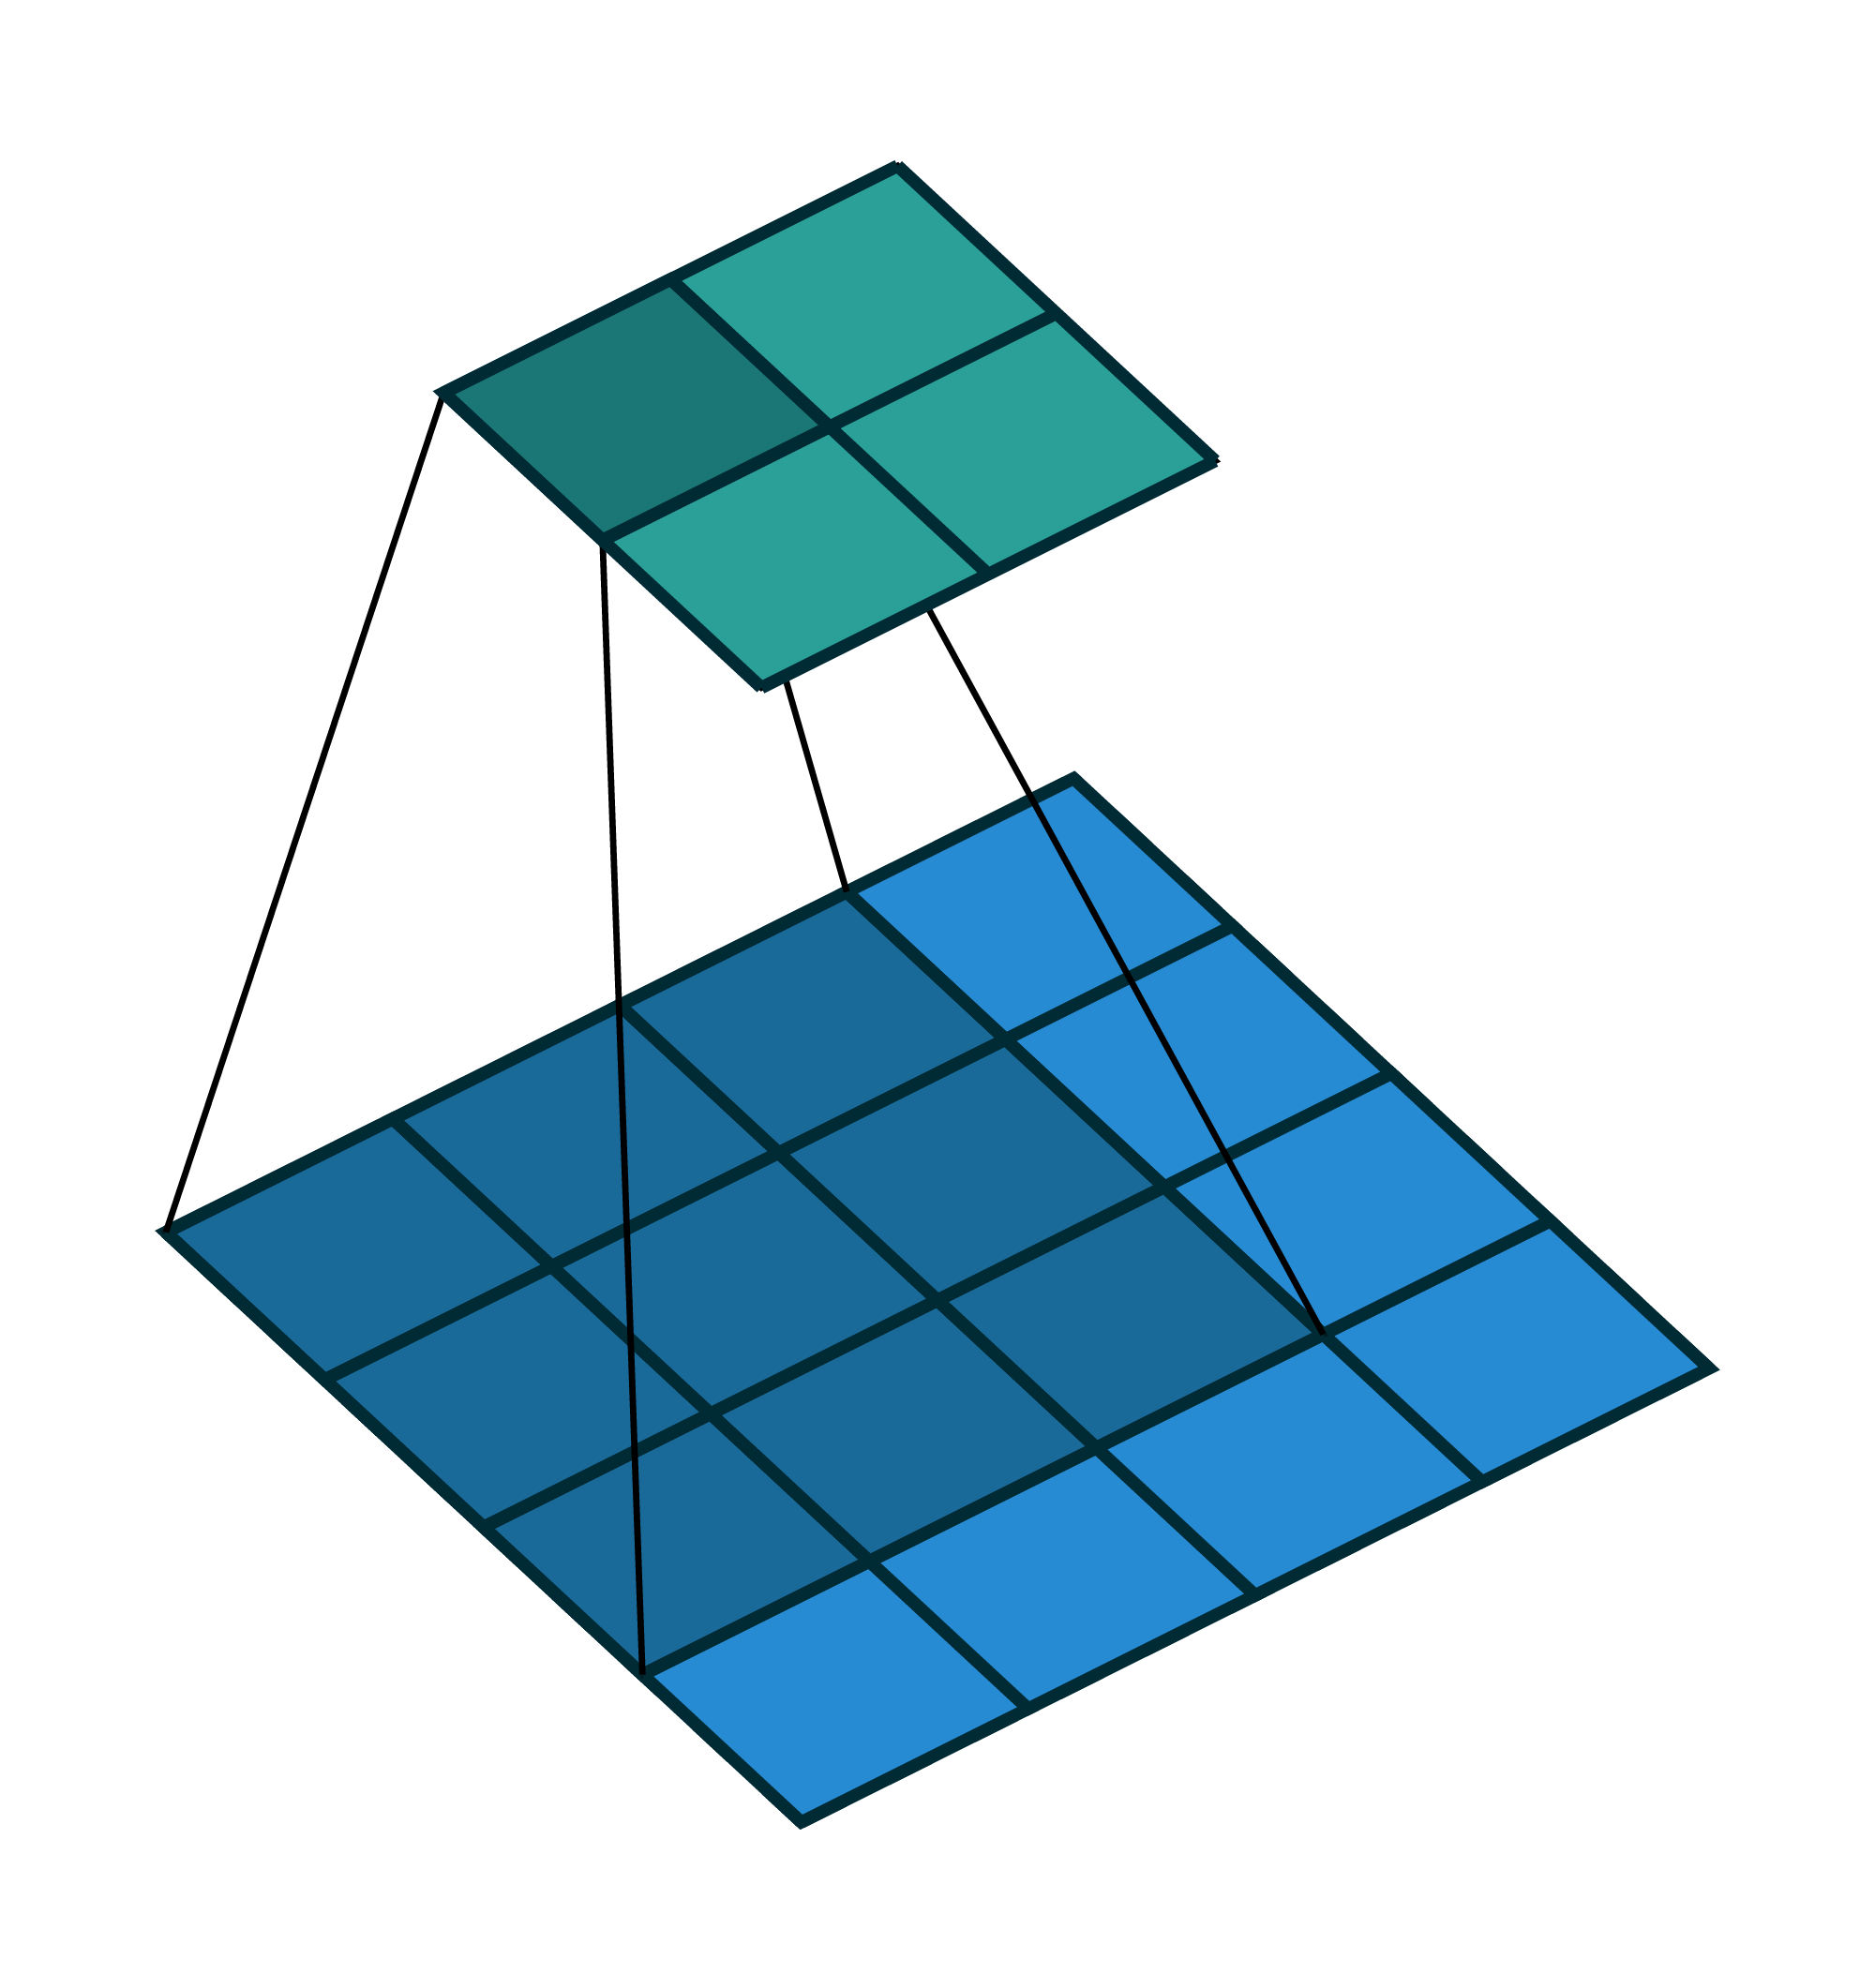
\includegraphics[width=.8\linewidth]{imgs/crbm_padding1.png}
  		\caption{The upward pass in the convolutional RBM}
  		\label{fig:convrbmsub1}
	\end{subfigure}%
	\begin{subfigure}[t]{.30\textwidth}
  		\centering
  		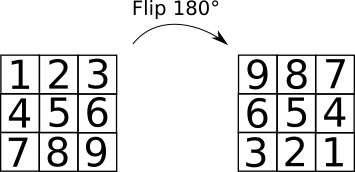
\includegraphics[width=.8\linewidth]{imgs/kernel_flip.png}
  		\caption{The 180\textdegree  flipped of the kernel matrix}
  		\label{fig:convrbmsub2}
	\end{subfigure}
	\begin{subfigure}[t]{.30\textwidth}
  		\centering
  		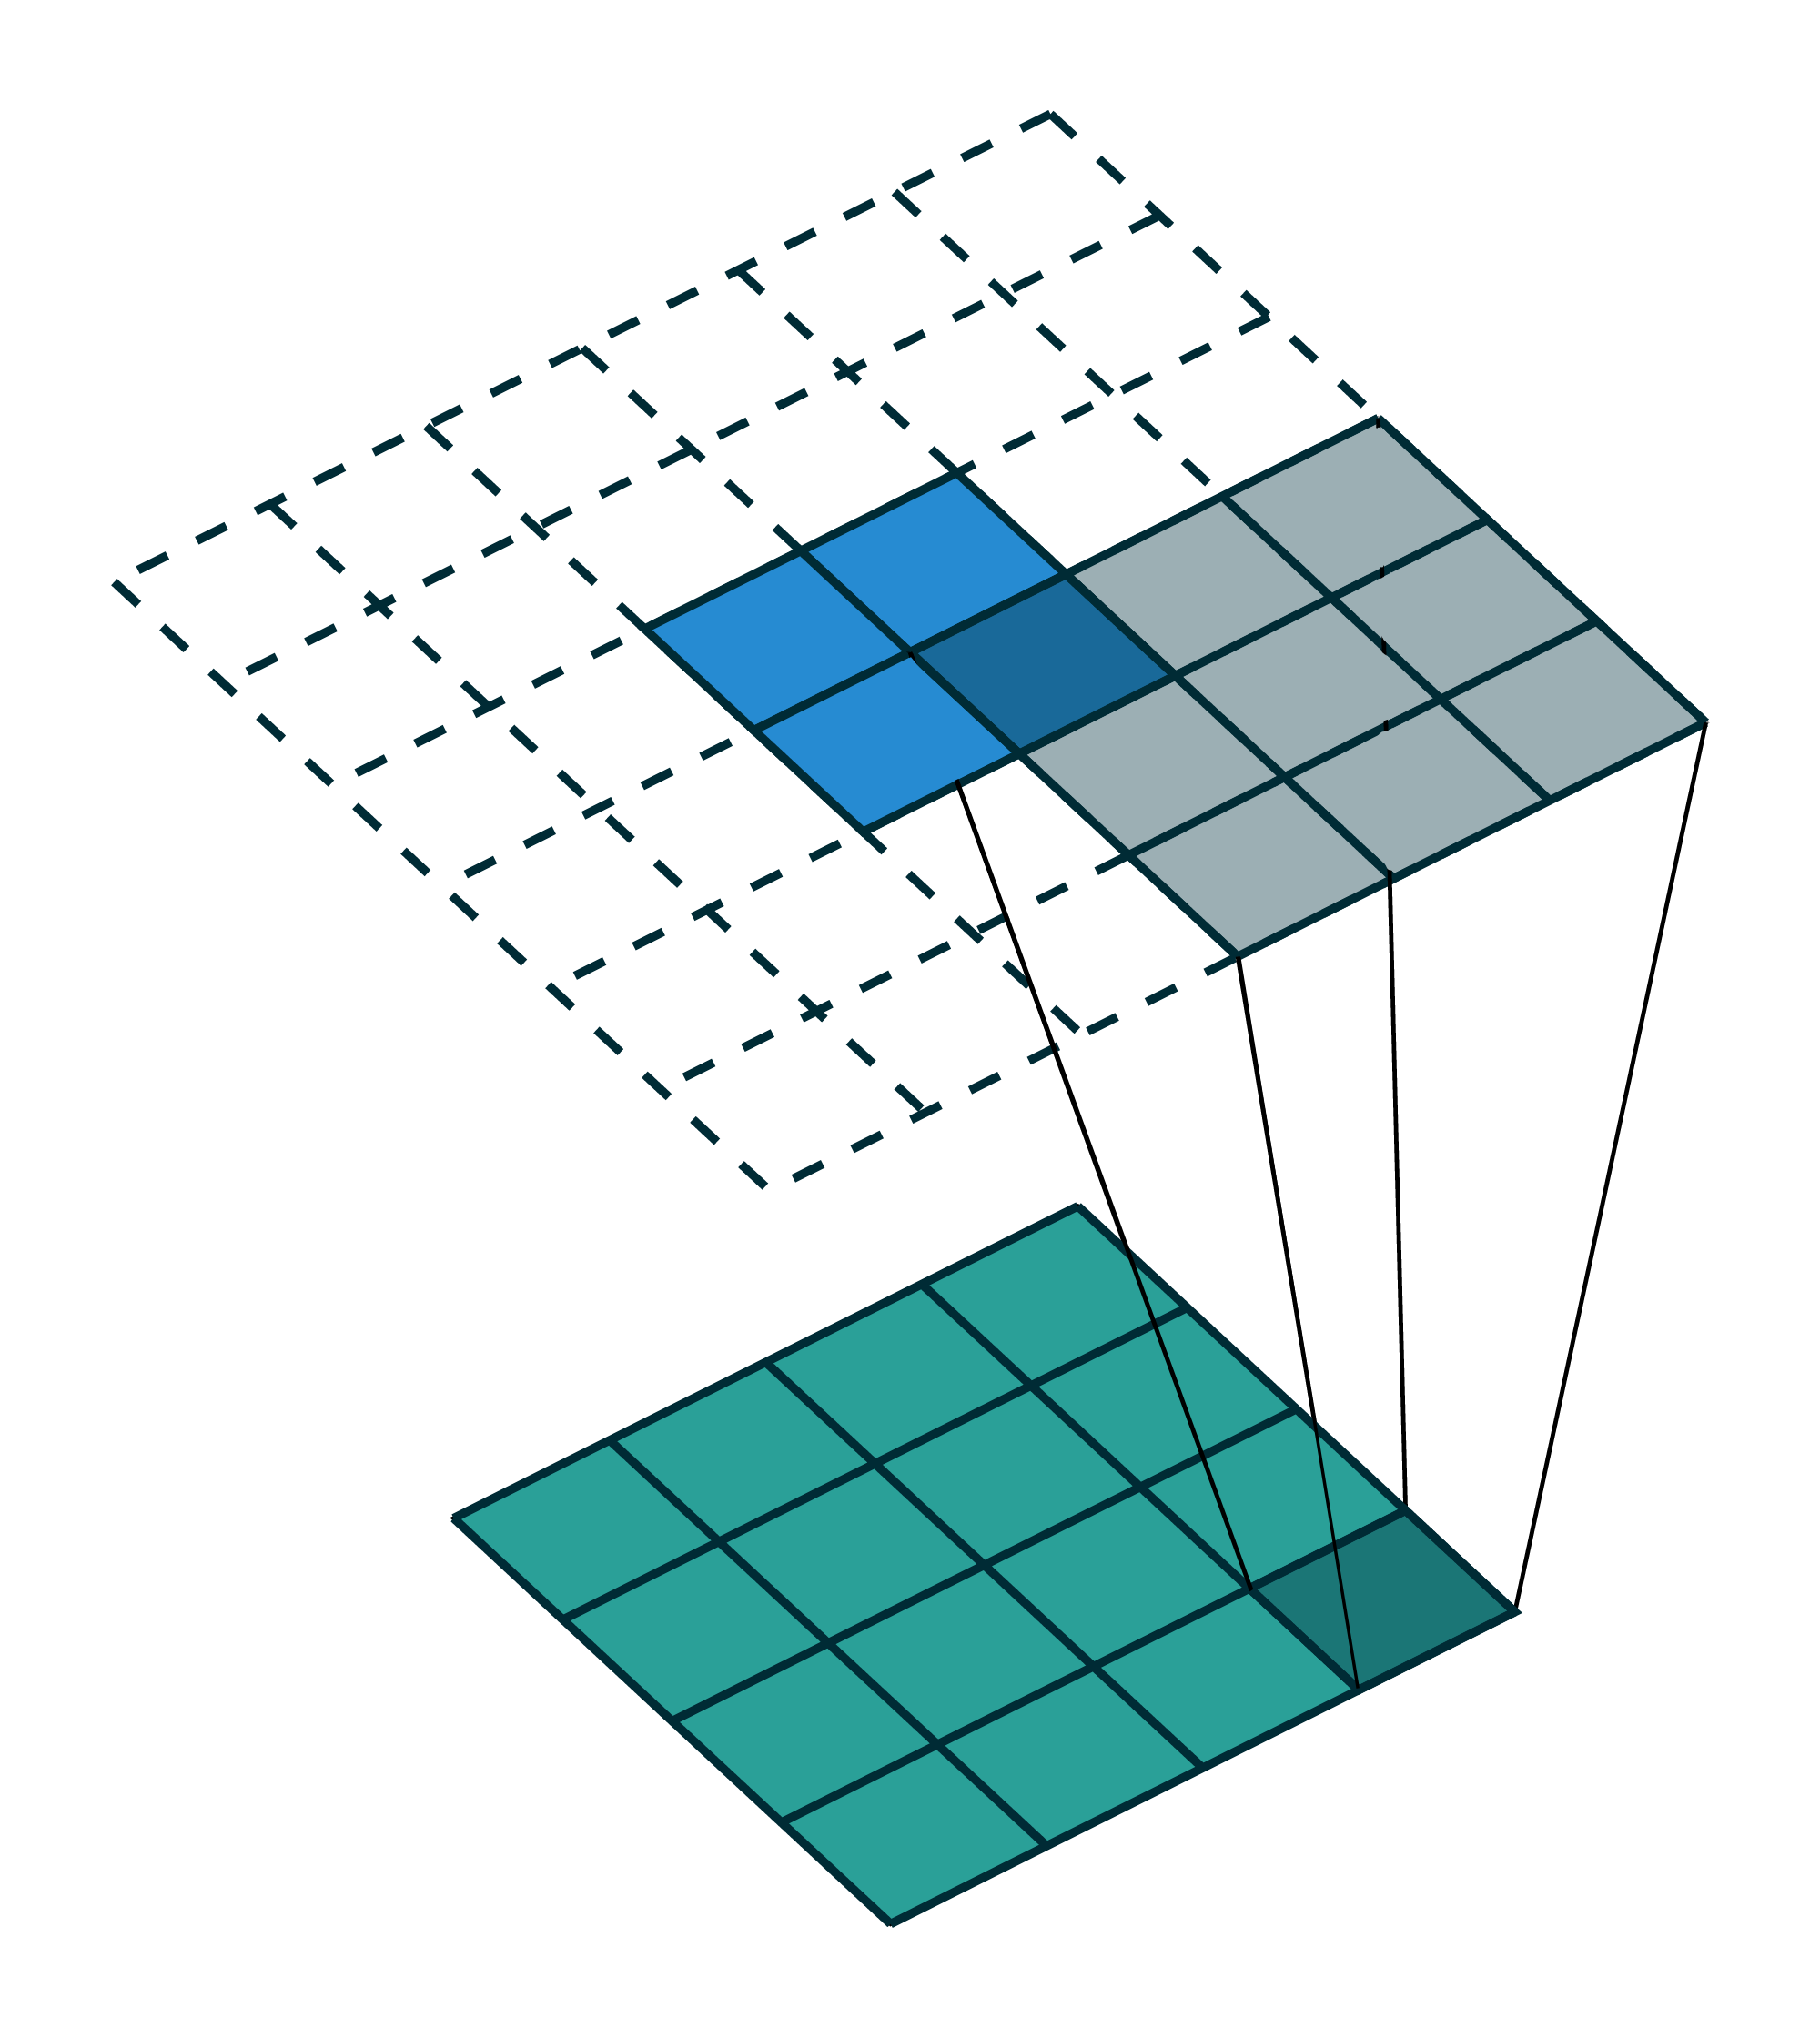
\includegraphics[width=.8\linewidth]{imgs/crbm_padding2.png}
  		\caption{The downward pass in the convolutional RBM}
  		\label{fig:convrbmsub3}
	\end{subfigure}
	\caption{A Gibbs sampling step in a convolutional RBM. At first the visible data is convolved with the kernel to get the hidden activations. Afterwards the kernel matrix is flipped 180\textdegree . In the downward pass the hidden activations with padding are convolved with the flipped kernel to get the new visible activations.}
	\label{fig:convrbm}
\end{figure}


Similar to normal a RBM, a convolutional RBM is trained with the objective to maximize the probability of the training data.
This can be achieved using the CD algorithm with a few adaptations due to the tied weights (see backprop for CNNs) \cite{NorouziM2009}: 
\[
\frac{\partial E}{\partial w} = \sum_{w \in W_{\text{group}}} \Delta w,
\]
where $W_{\text{group}}$ is a group of weights tied to the same value.

In contrast to CNNs, due to their local learning rule, RBMs can not be explicitly trained to perform max pooling operations.
Thus Lee et al. proposed an softmax based probabilistic max pooling to introduce local sparseness in the hidden activations, on which a pooling layer can be stacked \cite{lee2009convolutional}:
\[
P(h^k_{ij} | \textbf{v}) = \frac{\exp(I(h^k_{ij}))}{1 + \sum_{(i',j') \in B} \exp(I(h^k_{i'j'}))},
\]
where $I(h^k_{ij})$ is the activation of the hidden unit before applying the sigmoid function ( $(W * \textbf{v}) + \textbf{b}_{h}$ ) and $B$ is a partition block containing unit $h^k_{ij}$. 
Such an architecture is visualized in Fig \ref{fig:probmaxpool}.
This drives the activity in a block to be sparse and likely only one or none unit a block will be active.

\begin{figure}
	\centering
    	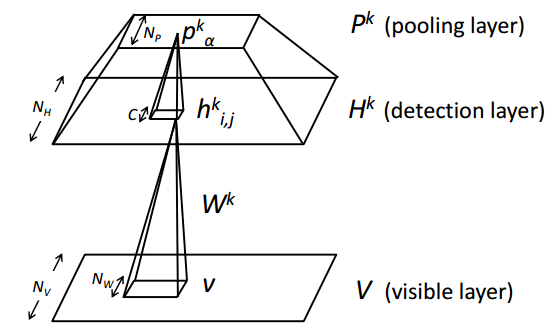
\includegraphics[width=0.4\textwidth]{imgs/prob_max_pool.png} 
    \caption{The RBM layer architecture with probabilistic max pooling \cite{lee2009convolutional}.}
	\label{fig:probmaxpool}
\end{figure}


\section{Sampling in SNNs}

Indicated by stochastic neural transitions found in the brain in experimental studies, a new way of information encoding in the brain as representations of probability distributions and probabilistic interference has been suggested \cite{lee2003hierarchical}\cite{yang2007probabilistic}\cite{griffiths2008bayesian}.


A first framework which proposed how spiking neurons can perform MCMC sampling was introduced by Buesing \cite{Buesing2011}.
A simplification to discretize time in time slices can be introduced without interfering with the basic concept (see Buesing for the generalization to continuous time \cite{Buesing2011}).

The neuron network can be considered as a network of RV, where the state of a neuron is defined by its firing. 
Since the probability of two neurons spiking at the same time is basically zero, after a neuron has fired it is set to the firing state for a time period $\tau$
\[
z_k(t) = 
\begin{cases}
1, &  \text{if k has fired in the time intervall } (t - \tau , t ] \\
0, &  \text{if k has not fired in the time intervall } (t - \tau , t ] 
\end{cases}
\] 
where $z_k$ is the state of neuron $k$ and set to $1$ for the "firing" state and $0$ for the "not firing" state (see Fig. \ref{fig:snnsamp1}). 
A common choice for $\tau$ is the refractory period of the neuron $\tau_{ref}$.
Consequently, one way to characterize the firing probability of a neuron is to take the ratio of the time a neuron has spent in state $z_i=1$ compared to the total timespan $T$ : $\frac{n_{\text{spikes}_i} \, \tau}{ T }$.

Thus for a given time step $t$ the state of the network $\textbf{z}(t) = (z_1(t), ... ,z_n(t))$ is defined by the state of the individual neurons $z_i(t)$. 


\begin{figure}
	\centering
    	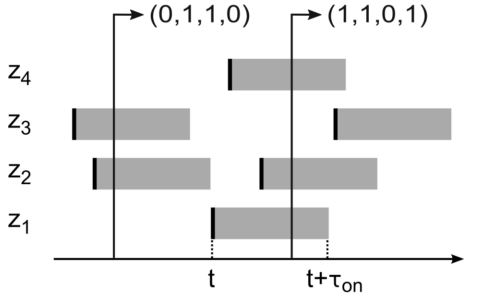
\includegraphics[width=0.4\textwidth]{imgs/snn_sample1.png} 
    \caption{A spiking neural network as probabilistic model. The state $z_i$ of a neuron is set to $1$ for a time period $t_{on}$ after a spike. The complete state of the network $\textbf{z}$ is given by the individual state $(z_1, z_2, z_3, z_4)$  \cite{Petrovici2016}.}
	\label{fig:snnsamp1}
\end{figure}

To get a process with Markovian properties $p(z_t| (z_0, ..., z_{t-1})) = p(z_t| z_{t-1}) $, a auxiliary counter variable $\xi \in \mathbb{N}$ is introduced which discretizes the time a neuron has left to stay in the "firing" state into time slices
\[
z_k(t) = 1 \iff \xi_k(t) \ge 1
\]
Thus $\xi$ can be seen as a counter, counting down from $\tau$ to $0$ in each time step after a neuron has fired (see Fig. \ref{fig:snnsamp2} for schematic overview and a sample implementation)
\[
p(\xi_t | \xi_{t-1}) = 
\begin{cases}
	1, & \text{ for } \xi_{t-1} > 1 \text{ and } \xi_t = \xi_{t-1} -1 ,\\
	p("firing"), & \text{ for } \xi_{t-1} \le 1 \text{ and } \xi_t = \tau ,\\
	p("not firing"), & \text{ for } \xi_{t-1} \le 1 \text{ and } \xi_t = 0 ,\\
	0, & \text{otherwise}.
\end{cases}
\]

\begin{figure}
	\centering
	\begin{subfigure}[t]{.39\textwidth}
  		\centering
  		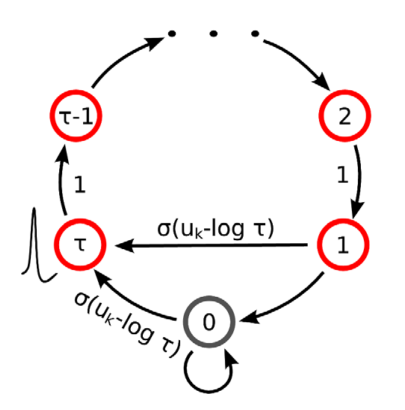
\includegraphics[width=0.9\textwidth]{imgs/snn_sample2.png}
  		\label{fig:snnsamp2sub1}
	\end{subfigure}
	\begin{subfigure}[t]{.59\textwidth}
  		\centering
  		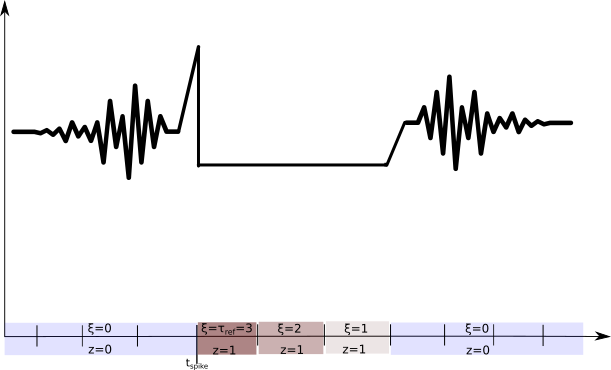
\includegraphics[width=0.9\textwidth]{imgs/sampl_bsp.png}
  		\label{fig:snnsamp2sub1}
	\end{subfigure}
    \caption{The artificial counter state $\xi$ of a neuron in a discrete time. In (a) the red state represent an active state $z_i = 1$. After a spike $\xi$ is set to the refractory period $\tau$. In each time step the refractory period counter $\xi$ is reduced by 1 until the neuron is inactive and can spike again. In (b) a exemplary membrane potential with the corresponding states of a neuron is given \cite{Buesing2011}.}
	\label{fig:snnsamp2}
\end{figure}




Buesing proposes an abstract stochastic neuron model which activates with a probability proportional to the input
\[
P(\textit{"i fires at time t"}) \approx \sigma(\sum_j w_{ij} z_j(t) + b_i).
\]
With this model Buesing proved that spikes and the corresponding state updates in a such networks can be seen as MCMC sampling. Experiments show, as $t \rightarrow \infty$ , the network is in fact able to approximate a Boltzmann distribution.
Replacing the rectangular PSP with a more biological plausible alpha shaped PSP deteriorates the performance a little, due to overshooting at the beginning and accumulation effects, but is still reasonable well (see Fig. \ref{fig:snnsamp3}).

\begin{figure}
	\centering
	\begin{subfigure}[t]{.50\textwidth}
  		\centering
  		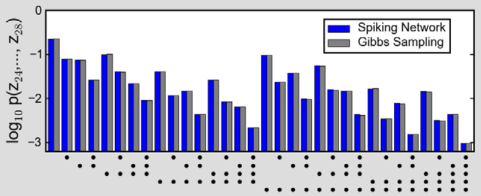
\includegraphics[width=.8\linewidth]{imgs/snn_sample3.png}
  		\caption{Sampling in a Boltzmann machine with a rectangular PSP kernel.}
  		\label{fig:sub1}
	\end{subfigure}%
	\begin{subfigure}[t]{.50\textwidth}
  		\centering
  		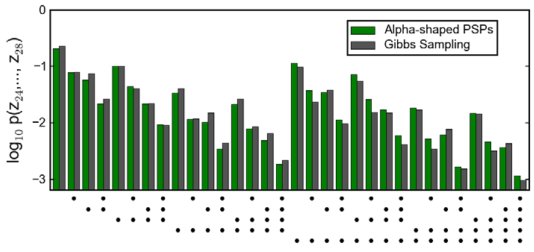
\includegraphics[width=.8\linewidth]{imgs/snn_sample4.png}
  		\caption{Sampling in a Boltzmann machine with a alpha-shaped PSP kernel. }
  		\label{fig:sub2}
	\end{subfigure}
	\caption{Comparison of the state probabilities with of neural sampling with Gibbs sampling in a four state Boltzmann machine. In (a) a probabilistic neuron model with a rectangular PSP is used and no discrepancies can be detected given a long enough sampling period. In (b) a more biological plausible alpha shaped kernel is used, which leads to some differences \cite{Buesing2011}.}
	\label{fig:snnsamp3}
\end{figure}

Petrovici improved the model by replacing the stochastic neuron model by conductance bases LIF neurons, a more common and biologically inspired neuron model \cite{Petrovici2016}.
He proved under high frequency (Poisson) noise, which leads to a high conductance state of the membrane potential, the neuron shows stochastic firing, determined by the input current and the noise frequency (as described in section 2.X).
This allows the neuron to show a firing behaviour which can be matched by a sigmoid function (see Fig. \ref{fig:snnsamp4}).  
By scaling the weights, the LIF neurons can be used to perform neural sampling similar to Buesing.

\begin{figure}
	\centering
    	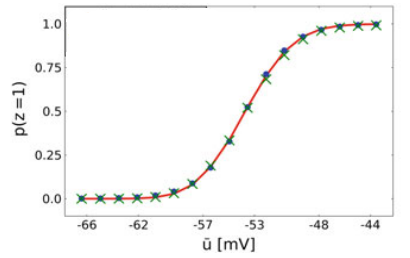
\includegraphics[width=0.4\textwidth]{imgs/snn_sample5.png} 
    \caption{Input output transfer function of a neuron in a high conductance state. The output rate is normalized by $\frac{1}{\tau_{ref}}$ to get a output probability. The transfer function is identical to shifted sigmoid function $\sigma$  \cite{Petrovici2016}.}
	\label{fig:snnsamp4}
\end{figure}

\section{Artificial to spiking neural network conversion}

The results of Petrovici allow a quite simple transformation of a Boltzmann machine to spiking neural networks of noisy conductance based LIF neurons with the synaptic weights scaled to match the impact on the membrane potential \cite{Petrovici2016}.
\\
\\
O'Connor uses a different approach, where instead of approximating sigmoid units by LIF neurons, he uses the Siegert neuron, a rate base approximations of LIF neurons with Poisson input, to implement units in the RBM which activate similarly to LIF neurons \cite{OConnor2013}. 
Such a trained net can be directly transferred to a SNN.
For a neuron its firing rate can be approximated by the Siegert transformation and can be normalized by the maximal firing rate to get an activation probability, which can be adapted by the units of the RBM. 
After the RBM with the Siegert activation function is trained, the weight can be simply adapted to a SNN with LIF neurons described by the Siegert approximation.
\\
\\
There also have been several approaches to transform a CNN to a SNN.  
Cao et al and Diehl et al propose certain constraints on the CNN architecture to show reasonable performance in the converted SNN \cite{Cao2014}\cite{Diehl2015}
\begin{itemize}
\item The CNN is only fed positive data since SNNs can't represent negative pre-synaptic spikes. 
\item The ReLU activation function is used in the CNN, which closely matches the input-output mapping of LIF neurons without a refractory period ( $t_{ref}=0$ ) and is always positive.
\item The bias term are eliminated.
\item Instead of max pooling, average pooling is used, since it has a simple spiking counterpart.
\end{itemize}
After the CNN is trained with the back propagation algorithm, the weights are transferred to a SNN with an equivalent architecture using LIF neurons without a refractory period (see Fig \ref{fig:csnnconv} for an adapted CNN the equivalent SNN architecture). 
In addition before applying the final weights, Diehl et al use some model- and data-based weight normalization procedure to further fine-tune the synaptic weights \cite{Diehl2015}. 

\begin{figure}
	\centering
	\begin{subfigure}[t]{.50\textwidth}
  		\centering
  		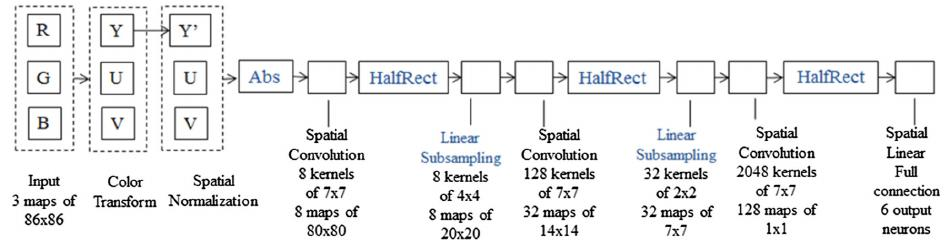
\includegraphics[width=.9\linewidth]{imgs/cnn_snn_conv1.jpg}
  		\caption{A for conversion adapted CNN architecture.}
  		\label{fig:sub1}
	\end{subfigure}%
	\begin{subfigure}[t]{.50\textwidth}
  		\centering
  		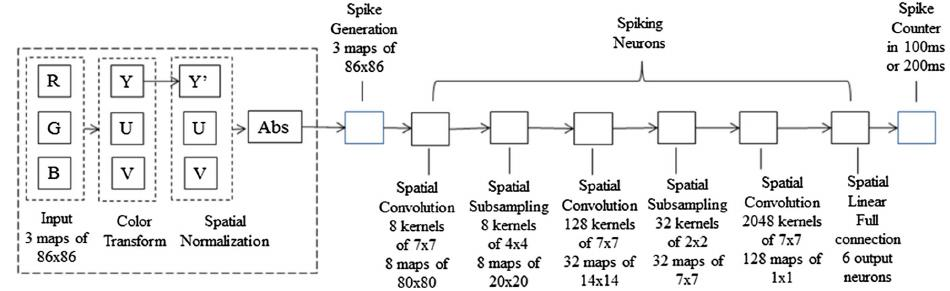
\includegraphics[width=.9\linewidth]{imgs/cnn_snn_conv2.jpg}
  		\caption{A to an SNN converted convolutional network.}
  		\label{fig:sub2}
	\end{subfigure}
	\caption{The proposed architectures to conversion between CNNs and SNNs \cite{Cao2014}. }
	\label{fig:csnnconv}
\end{figure}

\section{eCD and Sampling Machines}

Different approaches have been proposed to train a rate-based or spiking RBM, of which the first was probably by Hinton.
They use multiple identical binary stochastic input units for the each element in a data sample to approximate a rate based input \cite{Teh2005}.

The approaches described next make use of the synaptic sampling described in the previous chapter.

One approach is the evtCD by Daniel Neil which works in continuous time with spiking networks and a STDP variant \cite{Diehl2015}.
He simulates the positive and negative phase of the CD by unrolling the RBM with shared weights (a seen in Fig. \ref{fig:evtCD} where the RBM is unrolled to simulate CD-1 updates). 
But this approach only allows a fixed number of CD steps and is due to the weight synchronization not very plausible.

\begin{figure}
	\centering
    	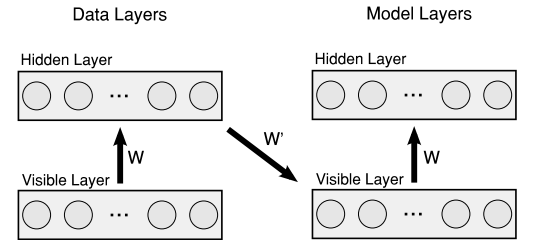
\includegraphics[width=0.4\textwidth]{imgs/evtCD.png} 
    \caption{An unrolled RBM with tied weights, which can be used to simulate the positive and negative phase and learn the weighs online \cite{Neil2013}.}
	\label{fig:evtCD}
\end{figure}

A more sophisticated approach, called eCD, which also uses STDP was proposed by Neftci \cite{Neftci2013}.
He uses bidirectional synapses, between a visible and hidden layer of LIF neurons.
They use an adapted symmetric STDP variant, which at a given time only allows LTP or LDP to model the positive or negative phase of the CD algorithm respectively (see Figure \ref{fig:ecdcomp} for a comparison). 
The symmetric learning rule for two neurons, given their spike train $v_i(t)$ and $h_j(t)$, can be expressed as:
\[
\Delta w_{ij} = \mu g(t) STDP(v_i(t), h_j(t)),
\]
with the learning rule $\mu$, the global STDP status flag $g(t)$ determining the positive and negative phase of the CD algorithm and the $STDP(v, h)$ parametrized to implement a symmetric weight change depended in the neural activity:
\[
\begin{split}
STDP(v_i(t), h_j(t)) = v_i(t) A_{h_j}(t) + h_j(t) A_{v_i}(t), \\
A_{h_j}(t) = A \int_{- \infty}^t W(t-s) h_j(s) ds, \\ 
A_{v_i}(t) = A \int_{- \infty}^t W(t-s) v_i(s) ds. \\ 
\end{split}
\]
In this STDP rule $A(t)$ can be seen as an activity trace indicating recent activity and $v_i(t)$ , $h_j(t)$ as a control variable enabling weight changes given a spike at time $t$.    
The kernel function $W$ should be symmetric, a common choice is $W(x) = exp(\frac{x}{\tau})$. 

\begin{figure}
	\centering
    	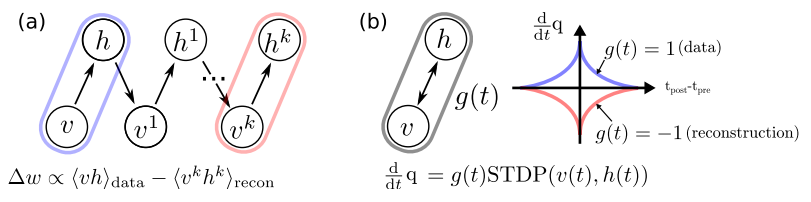
\includegraphics[width=0.8\textwidth]{imgs/eCD2.png} 
    \caption{Comparison between classical CD and event-based CD. In the classical k-CD (a) the weight update is determined by positive phase and negative phase, while in event-base CD (b) the weight update is determined by STDP and the sampling phase, determined by $g$ \cite{Neftci2013}.}
	\label{fig:ecdcomp}
\end{figure}
  
In their approach a training step can be divided into four phases (see Fig. \ref{fig:ecdph}):
\begin{enumerate}
\item The data signal is applied and the system is allowed to model the data distribution ($g(t)=0$)
\item Positive STDP is used to get $v_i h_j$-data (with LTP) and is added to the weights (postive phase $g(t)=1$)
\item The data signal is remove and the system is allowed to model the model distribution ($g(t)=0$)
\item Negative STDP is used to get $v_i h_j$-model (with LTD) and is subtracted from the synaptic weights (negative phase $g(t)=-1$).
\end{enumerate}


\begin{figure}
	\centering
    	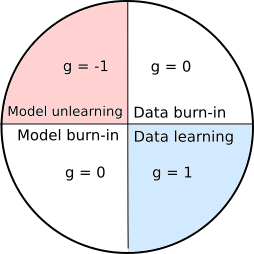
\includegraphics[width=0.3\textwidth]{imgs/eCD11.png} 
    \caption{Visualization of the phases of the event based contrastive divergence.}
	\label{fig:ecdph}
\end{figure}

In similarity to RBMs, the weight change in the second phase can be summarized as $\mu \; \delta w_{pos}$, the weight change in the fourth phase as $\mu \; \delta w_{neg}$, which results in the CD update rule:
\[
w = w +  \mu \; \delta w_{pos} - \mu \; \delta w_{neg} = w +  \mu (\delta w_{pos} - \delta w_{neg}).
\]
 